\begin{figure}[H]
    \centering
    
\includegraphics[width=0.5\textwidth]{figure/QR.png}
\end{figure}	

% \section{Dataset}
% Ini merupakan dataset yang digunakan dalam penelitian ini. Dataset ini diambil secara langsung dengan menggunakan kamera.
% \begin{figure}[H]
%     \centering
%     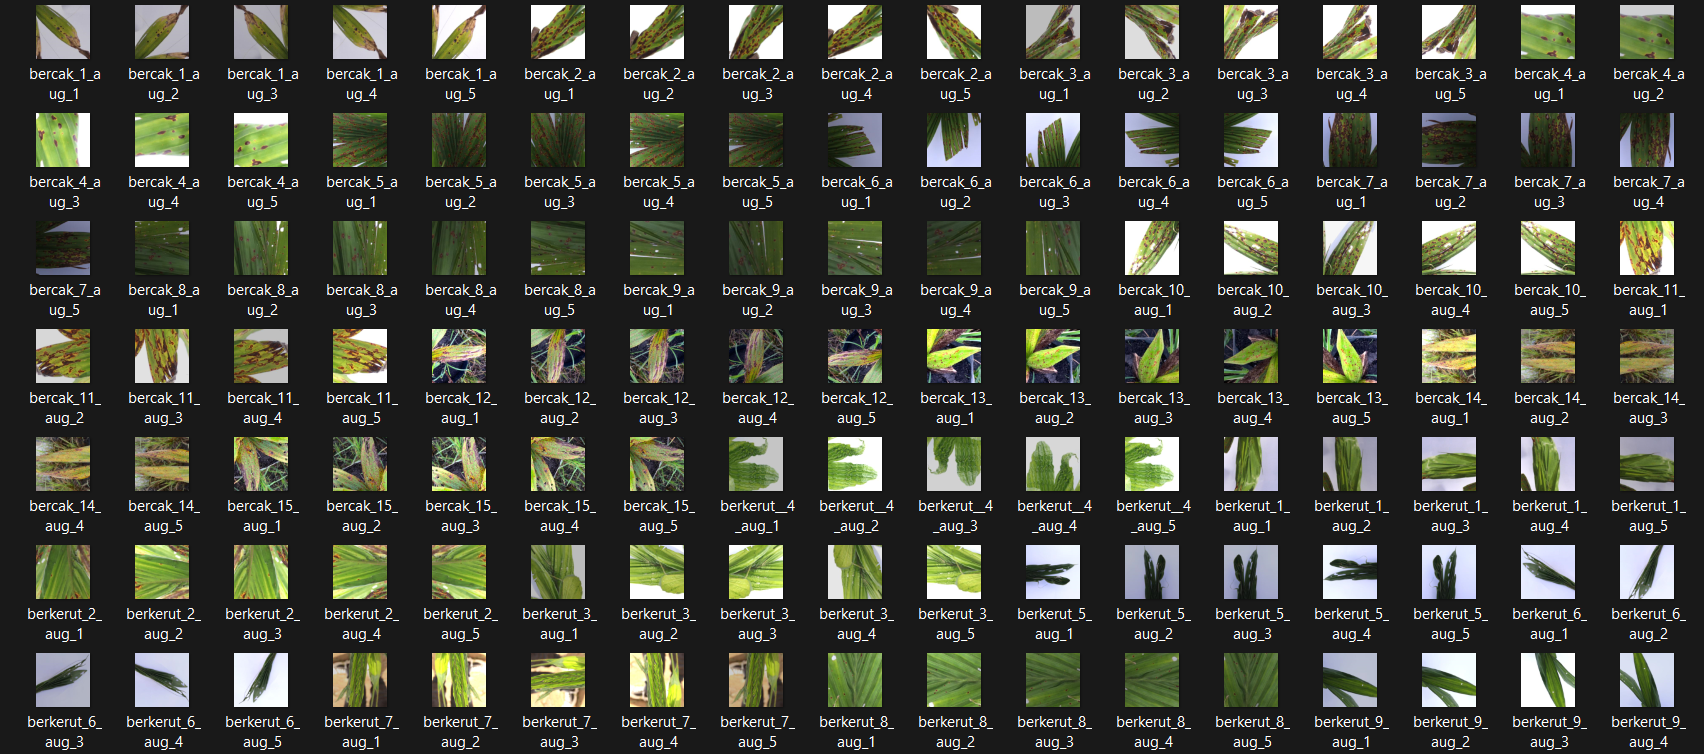
\includegraphics[width=1\textwidth]{figure/dataset-1.png}
%     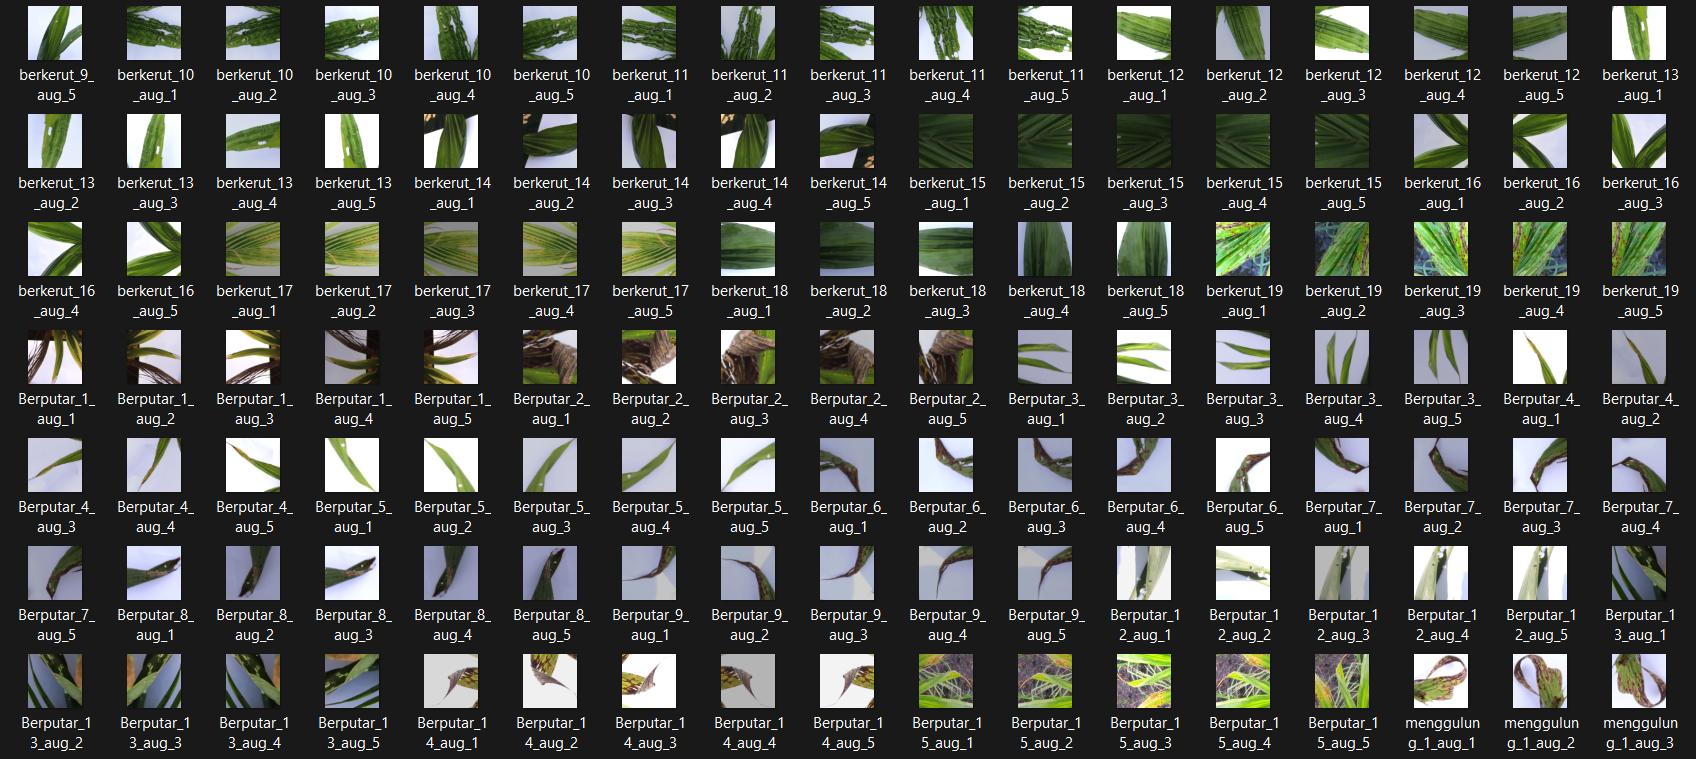
\includegraphics[width=1\textwidth]{figure/dataset-2.png}
%     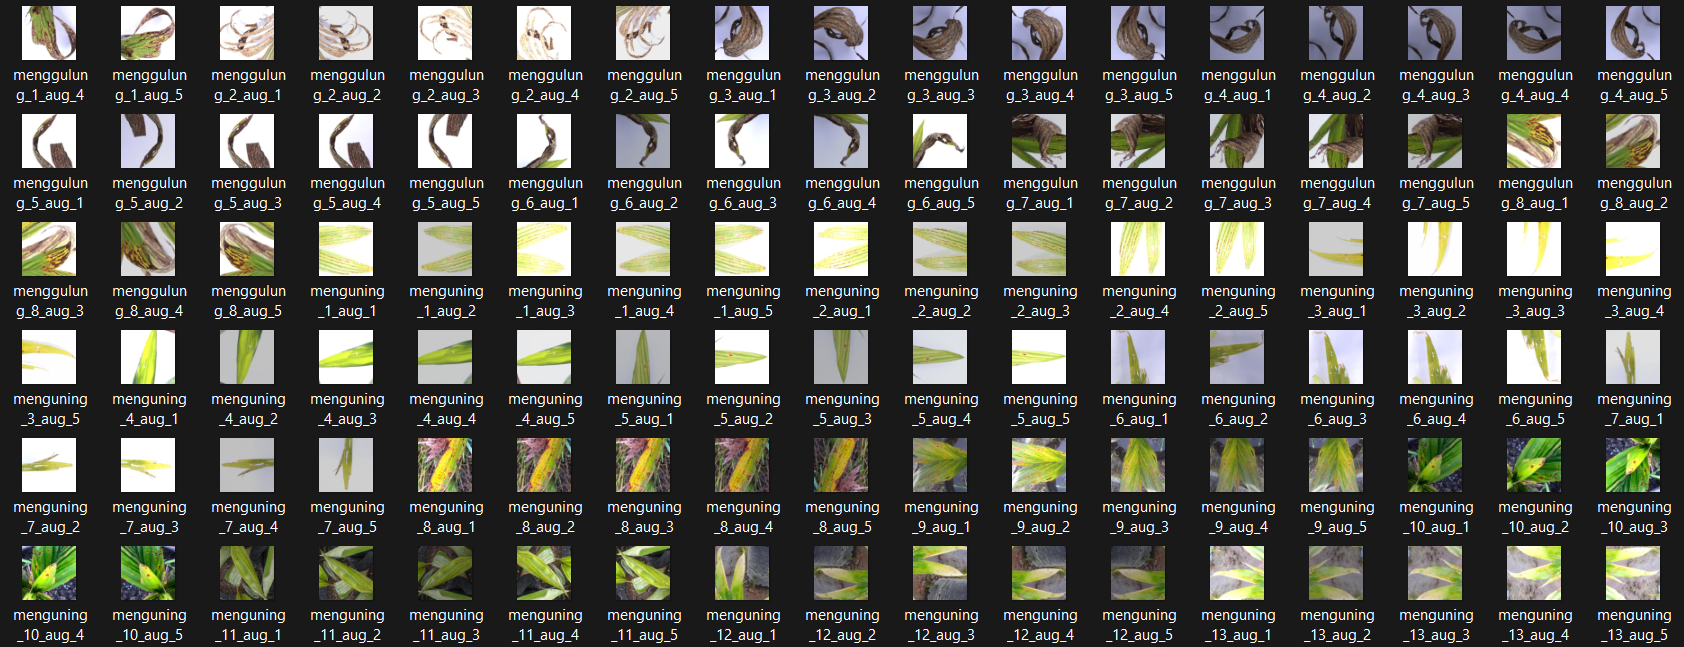
\includegraphics[width=1\textwidth]{figure/dataset-3.png}
% \end{figure}	


% \section{Dokumentasi Kegiatan}
% \begin{enumerate}
%     \item Wawancara dengan pihak PT. Perkebunan Nusantara IV Regional 7 Kebun Bekri untuk mendapatkan data yang dibutuhkan.
%     \begin{figure}[H]
%         \centering
%         \begin{minipage}{0.48\textwidth}
%             \centering
%             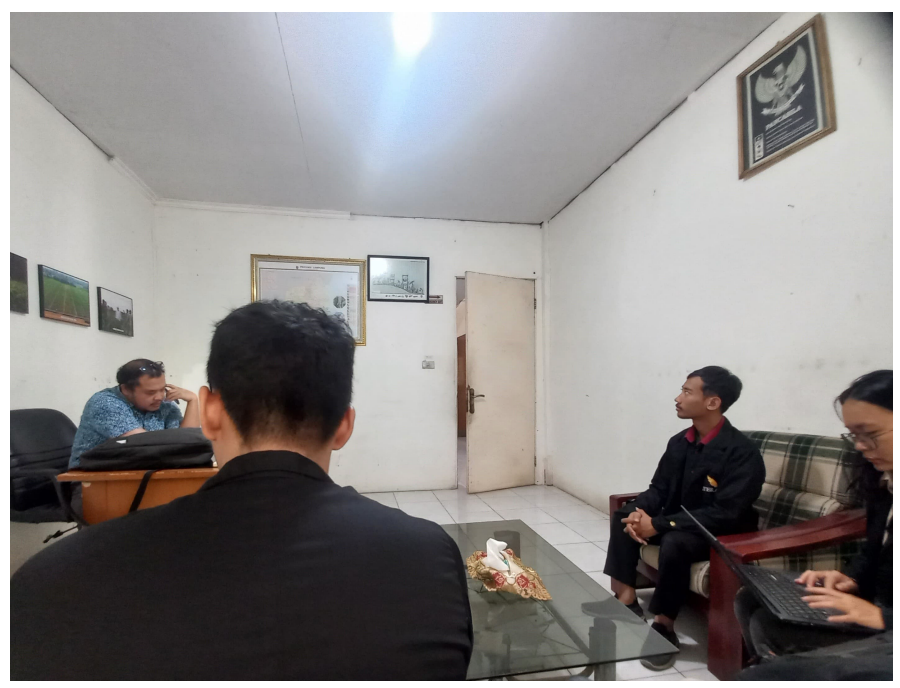
\includegraphics[width=\linewidth]{figure/wawancara-1-kantor.png}
%         \end{minipage}
%         \hfill
%         \begin{minipage}{0.48\textwidth}
%             \centering
%             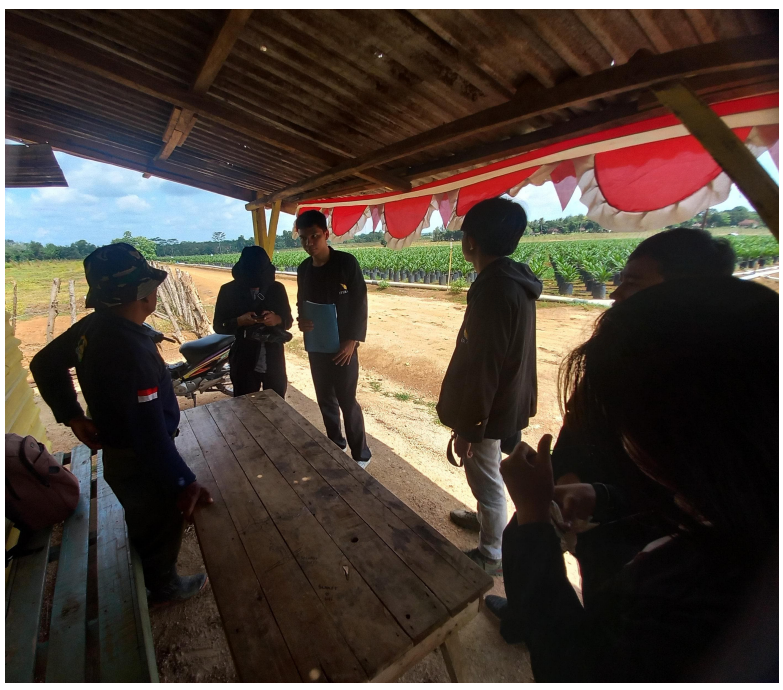
\includegraphics[width=\linewidth]{figure/wawancara-2-lapangan.png}
%         \end{minipage}
%     \end{figure}	

%     \item Pengambilan Dataset/Akuisisi Dataset dengan salah satu perwakilan dari PT. Perkebunan Nusantara IV Regional 7 Kebun Bekri, yaitu Bapak Wahab pada tanggal 28 Oktober dan 06 November 2024.
%     \begin{figure}[H]
%         \centering
%         \begin{minipage}{0.48\textwidth}
%             \centering
%             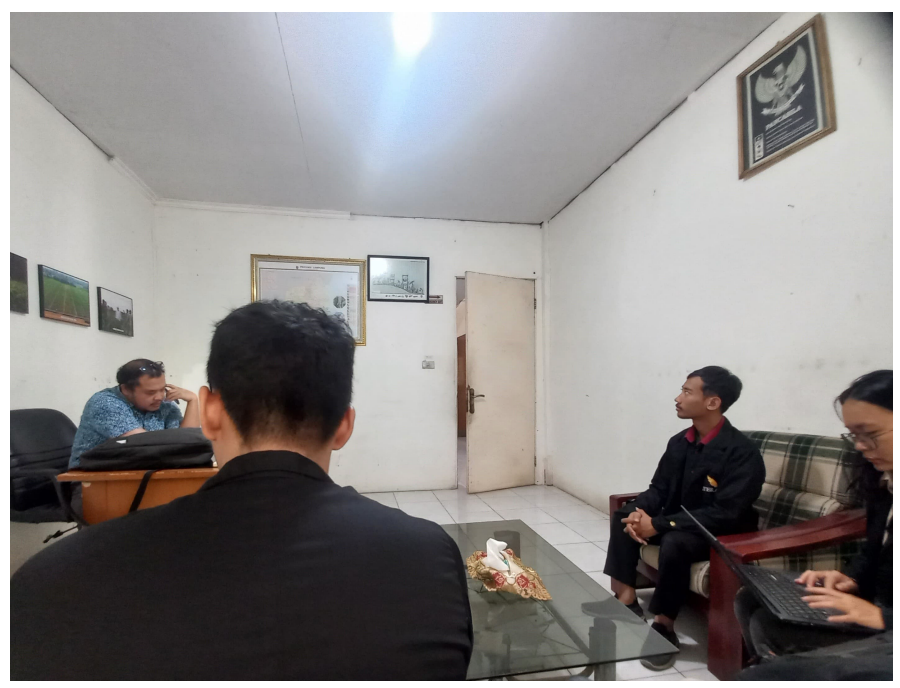
\includegraphics[width=\linewidth]{figure/wawancara-1-kantor.png}
%         \end{minipage}
%         \hfill
%         \begin{minipage}{0.48\textwidth}
%             \centering
%             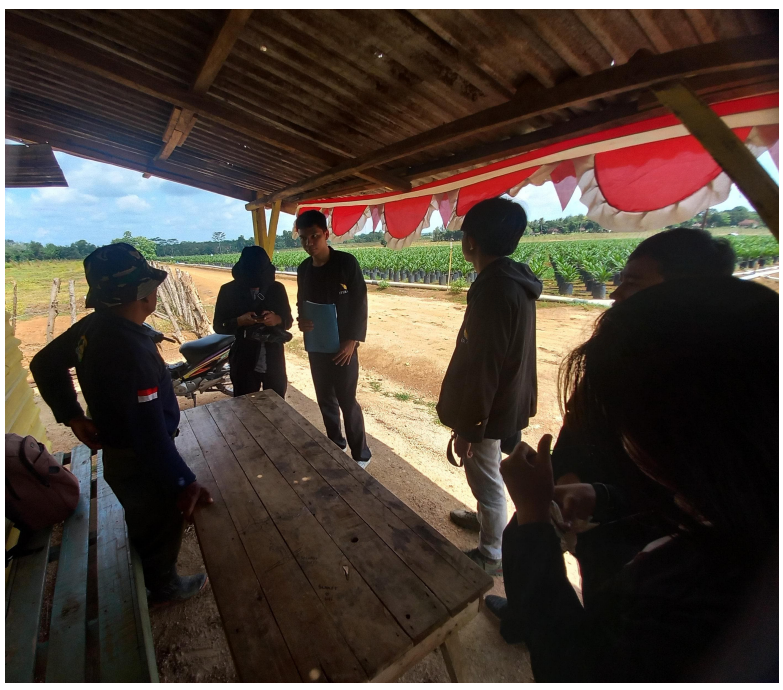
\includegraphics[width=\linewidth]{figure/wawancara-2-lapangan.png}
%         \end{minipage}
%     \end{figure}	

%     \item Evaluasi hasil penelitian dan pembuatan laporan akhir.
% \end{enumerate}



% % \section{Rincian Kasus Uji}
% % \begin{figure}[H]
% %     \centering
% %     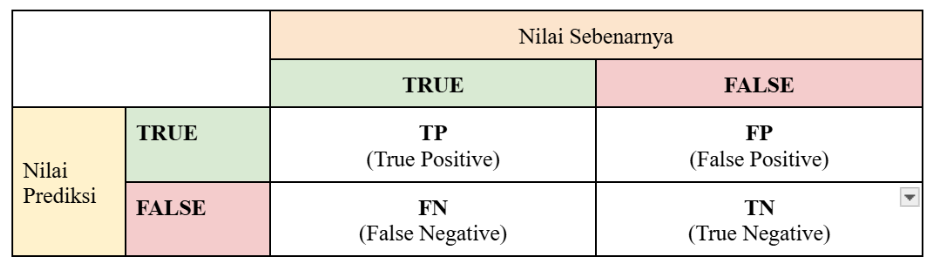
\includegraphics[width=0.5\textwidth]{figure/chapter-2-Confusion-Matrix.png}
% %     \caption{Confusion Matrix}
% %     \label{fig:2.ConfusionMatrix}
% % \end{figure}	